\section{System Architecture}


\begin{figure}[t]
    \centering
    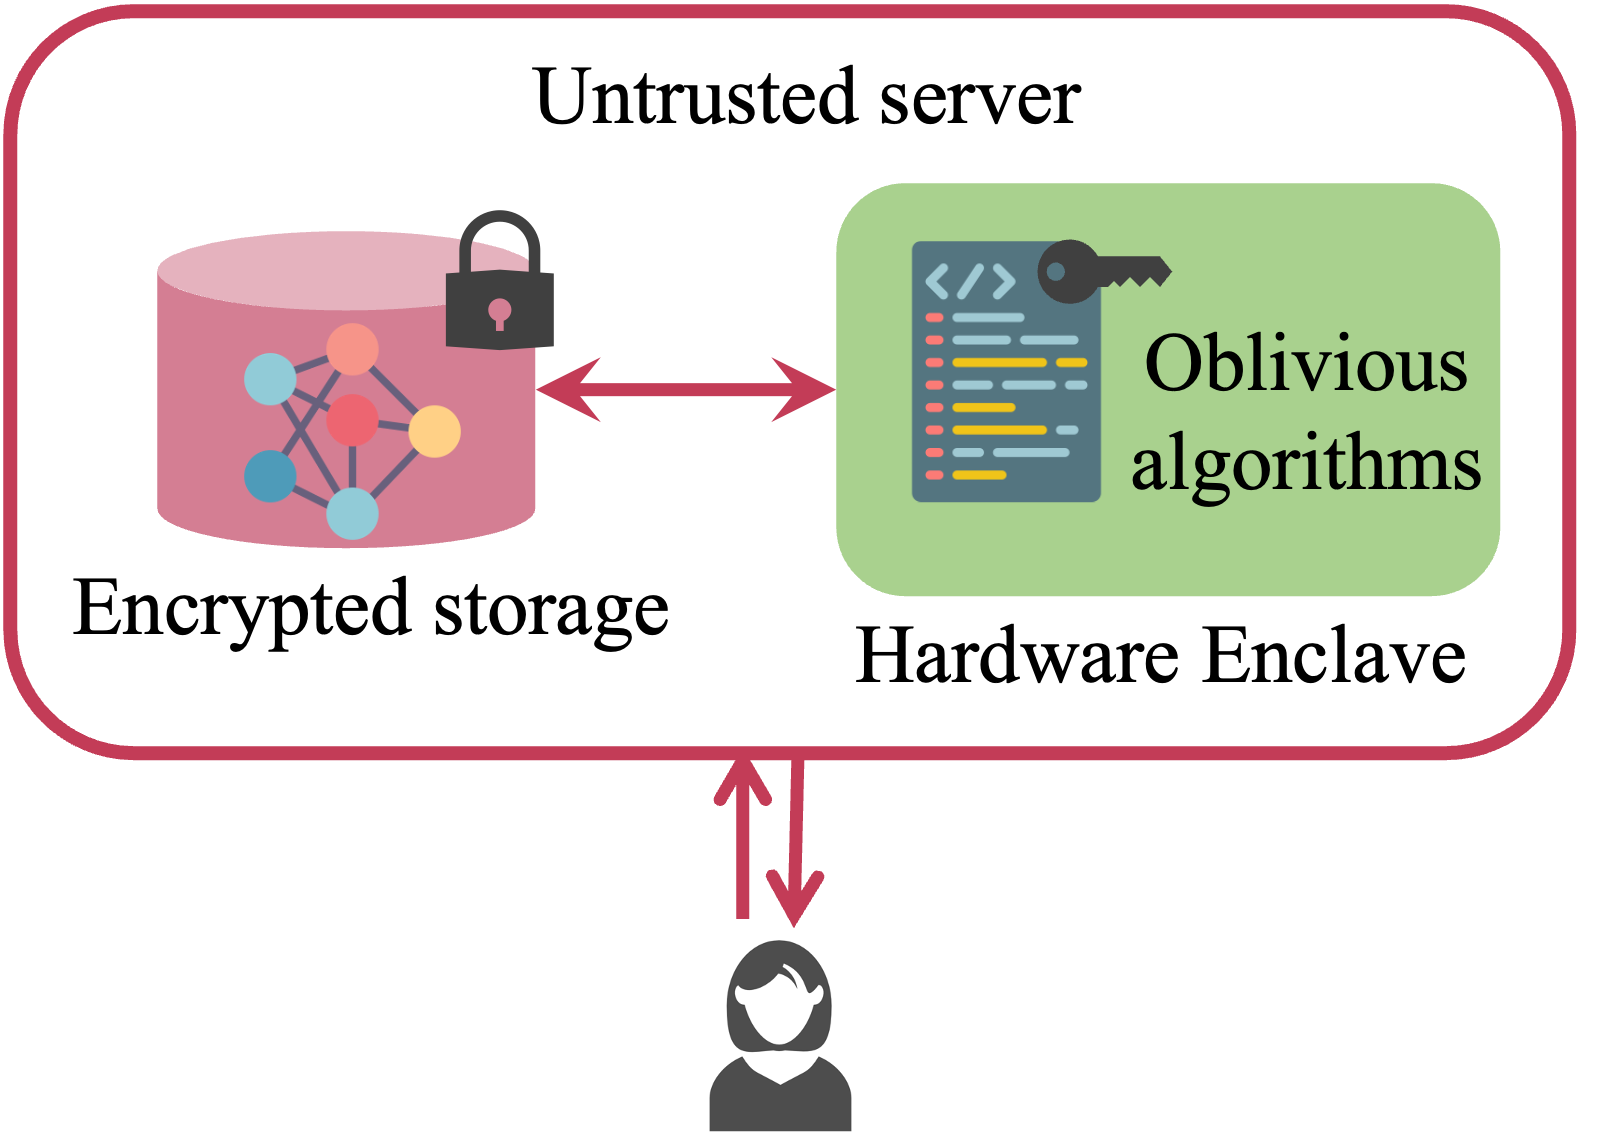
\includegraphics[scale=0.4]{figures/system-model.png}
    \vspace{-1em}
    \caption{\centering System architecture of an enclave-based oblivious graph database} 
    \label{fig:sys-model}
    \Description{}
    \vspace{-1em}
\end{figure}


We consider an architecture where an application, acting as the data owner, 
outsources its data storage and computation to a cloud provider, as 
illustrated in Figure~\ref{fig:sys-model}. The data is structured as a 
property graph, consisting of multiple types of nodes, called \textit{node 
labels}, connected by one or more types of edges, called \textit{edge 
labels}. To protect data privacy from a potentially untrusted cloud 
provider, the data owner encrypts the graph using secure encryption schemes 
such as AES before outsourcing it. Clients, considered to be trusted and 
hence have permissions to query the data, send Cypher~\cite{opencypher} queries to the 
server. An oblivious graph database program running within a hardware 
enclave processes client requests by retrieving encrypted data from persistent 
cloud storage (e.g., AWS S3 buckets) and executes oblivious query processing
algorithms.


\subsection{Threat Model}

%\noindent\textbf{\underline{Threat model}}: 
In discussing the challenges and future 
research directions for oblivious graph databases, we adopt a commonly used 
threat model in enclave-based approaches~\cite{dauterman2021snoopy, krastnikov2020efficient, mishra2018oblix, chamani2023graphos, mavrogiannakis2025obliviator}, where 
the attacker can observe the server's encrypted network traffic, manage the 
software stack outside the enclave, and monitor memory accesses both inside 
and outside the enclave at cache line granularity. However, the adversary 
cannot breach the secure processor or access its secret key. The attacker 
may leverage observable information to launch side-channel attacks, including cache attacks~\cite{brasser2017software, hahnel2017high, moghimi2017cachezoom, schwarz2017malware}, branch prediction and
paging-based attacks~\cite{lee2017inferring, van2017telling, xu2015controlled}, 
and memory bus snooping~\cite{lee2020off}. Attacks based on power 
consumption and timing analysis are considered out of scope for this model.

In protecting data from such an adversary, oblivious systems often consider 
certain information about the data to be public and do not attempt to hide 
it from the adversary. For instance, oblivious RDBMSs allow public 
knowledge of the schema, the number of tuples per table, the type of 
queries executed by clients, and the final output 
size~\cite{mavrogiannakis2025obliviator, krastnikov2020efficient, popa2011cryptdb, eskandarian2019oblidb}. Similarly, 
GraphOS~\cite{chamani2023graphos} exposes equivalent information for graph data. In the context of an oblivious property graph database, we consider 
the number of nodes and edges per label, the type of query executed by 
clients, and the final query output size as public information. However, 
any intermediate output size must remain hidden from the adversary.
% , which presents a significant challenge in the design of an oblivious graph database.

% \rjm{depending on space, you might add an example of an intermediate size for a graph query that is clearly revealing information.  And if it is in a way a relational query wouldn't leak information, that would be great.}

\subsection{Data Model}
\label{sub:data-model}
We model the property graph~\cite{robinson2015graph} data with nodes, edge
relationships, and properties, similar to plaintext graph databases.
\begin{itemize}[leftmargin=*]
    \item \textbf{Node:} Each node type, identified using a
    \textit{label}, represents an entity in the data. Within each node label, we identify discrete nodes using a unique numerical id starting from 0.
    \item \textbf{Edge relationship:} An edge relationship,
    referred to simply as edges here onward, represents a connection between nodes (either of same or different labels). Similarly to the nodes, each edge type is identified by
    an \textit{edge label}. 
    %with each edge within a label identified by a unique numerical id starting from 0. 
    Each edge connects a source node to a destination node, and the edges are uni-directional. 
    %In this model, we restrict two nodes to be connected by unique edge labels.
    \item \textbf{Property:} Each node and edge label can consist of a number of properties, storing more descriptions about the data.
\end{itemize}

\subsection{Storage Model}
\label{sub:storage-layer}

Storage models used in existing oblivious databases pose unique
challenges for efficiently storing graph data. Current oblivious databases 
either store data in key-value format~\cite{dauterman2021snoopy, mishra2018oblix} or row-wise tabular format~\cite{zheng2017opaque,eskandarian2019oblidb,mavrogiannakis2025obliviator}. GraphOS~\cite{chamani2023graphos} stores graph 
data as key-values using an oblivious AVL tree, which incurs
$O(polylogN)$ overhead to access \textit{each node or edge} in the 
graph. This becomes a performance bottleneck with a graph of 
millions of nodes and edges. While graph data
can be stored in a row-wise tabular format, as seen in 
plaintext graph databases, such a storage model is inefficient 
for graph analytics. Hence, we advocate for a model that is conducive for graph analytics:
\textit{a disk-based columnar storage}, where each node or edge 
property will be stored in a separate column file.  

\begin{figure}[t]
    \centering
    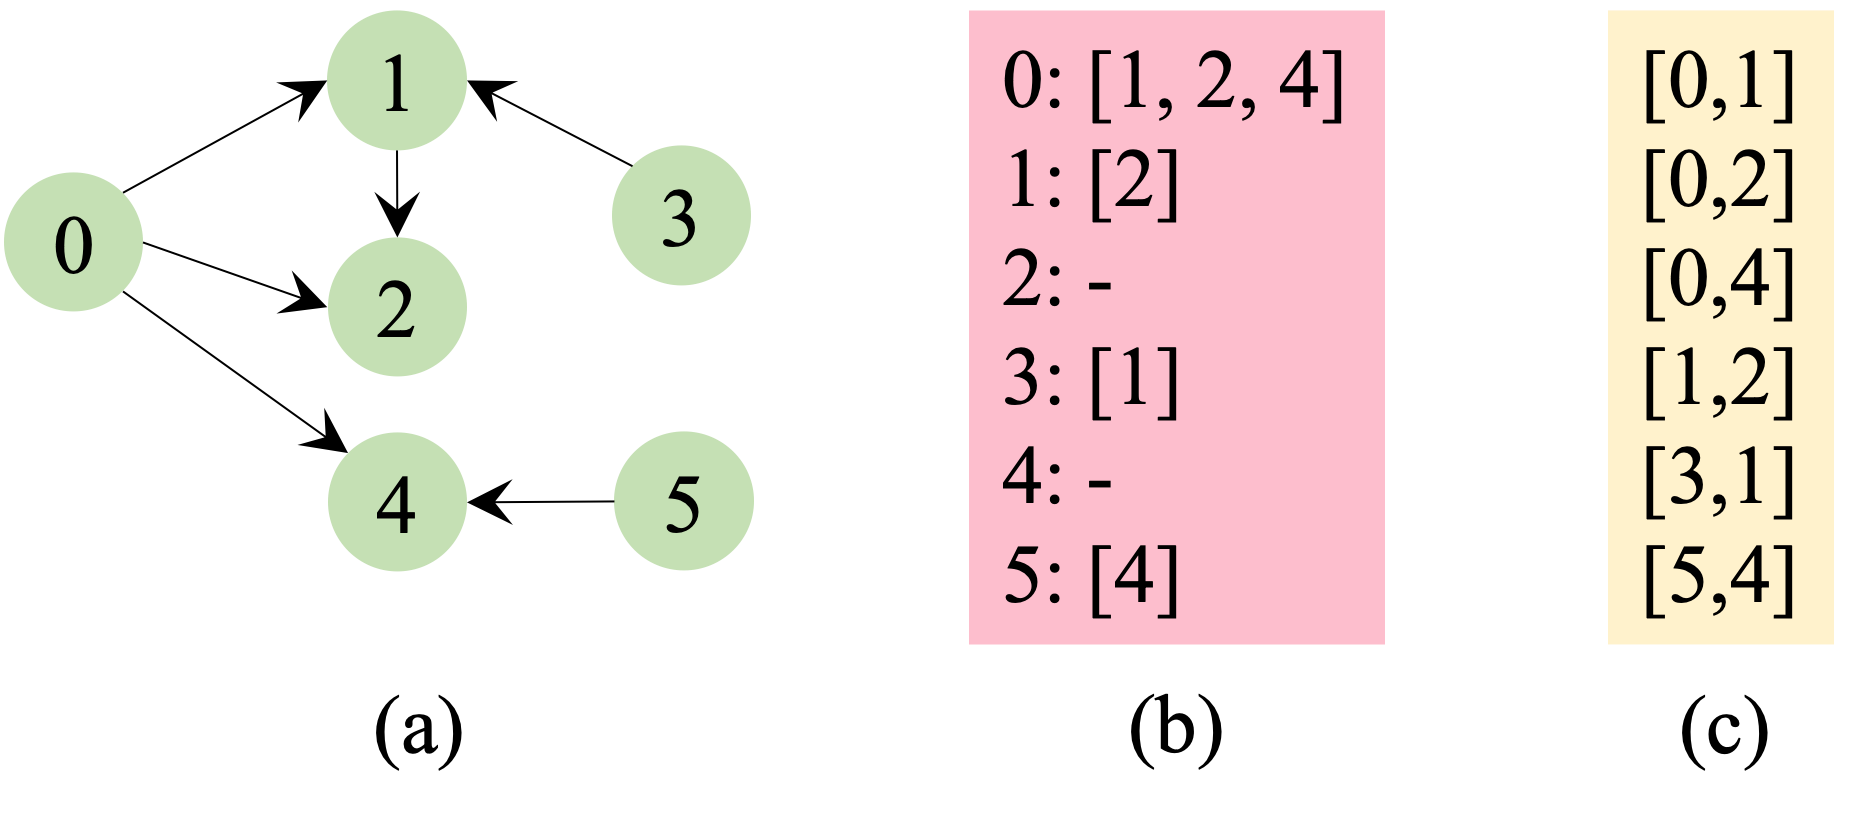
\includegraphics[scale=0.4]{figures/edge_storage.png}
    \vspace{-1em}
    \caption{\centering (a) Sample graph data. (b) Insecure edge representation. (c) Secure edge storage. } 
    \label{fig:edge-storage}
    \Description{}
    \vspace{-1em}
\end{figure}

Plaintext graph databases typically store the edges using an
adjacency list, as seen in Figure~\ref{fig:edge-storage}(b). However, this representation
is insecure because it reveals the degree of
each node, even when the ids are encrypted. Hiding this information
would require padding the adjacency list to a size of
$m\times n$, where $m$ is the number of edges and $n$ the nodes, because
in the worst case, all $m$ edges can originate from a single
node. Therefore, we propose to store the adjacency in a single
array-like format, sorted on the ids of the source nodes
as shown in Figure~\ref{fig:edge-storage}(c). This only exposes $m$, the number of edges (of
a particular label), which is considered non-sensitive. 
Additionally, similar to plaintext graph databases designs such as~\cite{janusgraph,feng2023kuzu,deutsch2019tigergraph,sun2015sqlgraph}, we recommend maintaining \textit{reverse edges}
stored in the sorted order of destination node ids (also of size $m$) to enable 
bi-directional parallel processing of graph queries. While many plaintext 
graph databases use columnar storage and forward-\&-reverse edge lists,
to our knowledge, we are the first to deviate from the key-value or tabular format in oblivious databases.


% \rjm{Has the secure storage (2(c)) proposed here been used before?  I'm wondering about novelty and if this specific representation allows reverse edges that are secure (don't reveal information).?}